\section{Spatial Readout Interface and Qualification Gate}
\label{app:readout}

\begin{figure*}[!t]
\centering
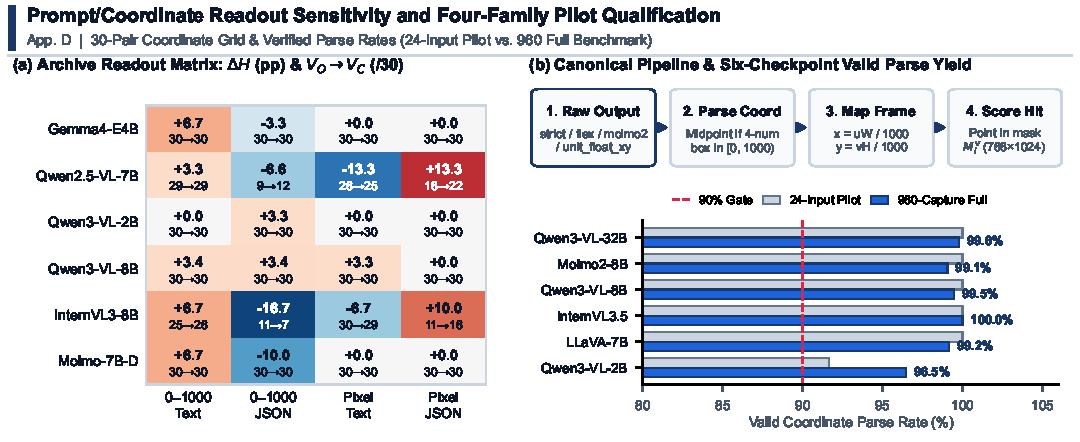
\includegraphics[width=0.95\textwidth]{app_fig3_readout_and_pilot.pdf}
\caption{\textbf{Spatial readout frame sensitivity and four-family pilot qualification.}
\emph{(a)} Archive heatmap of paired score deltas $\Delta H = H_C - H_O$ (percentage points) and valid numeric parse counts $(V_O \to V_C / 30)$ across normalized $0\text{--}1000$ vs.\ pixel frames and text vs.\ JSON prompts (full values in Table~\ref{tab:protocol-full}).
\emph{(b)} Canonical four-step \texttt{Parse $\to$ Align $\to$ Score} pipeline (top) and verified valid coordinate parse rates on both the isolated 24-input pilot qualification gate ($\ge 90\%$) and full 960-capture 30-scene benchmark ($96.5\%\text{--}100.0\%$ across all six evaluated checkpoints).}
\label{fig:app-readout-pilot}
\end{figure*}

Inconsistent prompt schemas or coordinate conventions can easily masquerade as optical sensitivity. Figure~\ref{fig:app-readout-pilot}(a) and Table~\ref{tab:protocol-full} evaluate six model configurations on fixed 30-pair target-centered captures across a $2{\times}2$ interface matrix crossing frame requests ($0\text{--}1000$ normalized vs.\ image pixels) and response schemas (two-line text \texttt{Point:\ x, y} vs.\ JSON \texttt{point\_xy}). A parsed point counts toward valid parse coverage $V$ even when falling outside image bounds, whereas a hit $H$ requires landing inside the target region.

\begin{table}[!htbp]
\centering\small
\setlength{\tabcolsep}{3pt}
\resizebox{\linewidth}{!}{% Generated by scripts/build_assets.py from corrected results.json
\begin{tabular}{lllrrrr}
\toprule
Model & Frame & Format & $V_O$ & $V_C$ & $H_O$ (\%) & $H_C$ (\%) \\
\midrule
Gemma4-E4B & 0--1000 & text & 30/30 & 30/30 & 90.0 & 96.7 \\
Gemma4-E4B & 0--1000 & JSON & 30/30 & 30/30 & 90.0 & 86.7 \\
Gemma4-E4B & pixel & text & 30/30 & 30/30 & 36.7 & 36.7 \\
Gemma4-E4B & pixel & JSON & 30/30 & 30/30 & 0.0 & 0.0 \\
Qwen2.5-VL-7B & 0--1000 & text & 29/30 & 29/30 & 10.0 & 13.3 \\
Qwen2.5-VL-7B & 0--1000 & JSON & 9/30 & 12/30 & 13.3 & 6.7 \\
Qwen2.5-VL-7B & pixel & text & 26/30 & 25/30 & 80.0 & 66.7 \\
Qwen2.5-VL-7B & pixel & JSON & 18/30 & 22/30 & 60.0 & 73.3 \\
Qwen3-VL-2B & 0--1000 & text & 30/30 & 30/30 & 86.7 & 86.7 \\
Qwen3-VL-2B & 0--1000 & JSON & 30/30 & 30/30 & 90.0 & 93.3 \\
Qwen3-VL-2B & pixel & text & 30/30 & 30/30 & 60.0 & 60.0 \\
Qwen3-VL-2B & pixel & JSON & 30/30 & 30/30 & 0.0 & 0.0 \\
Qwen3-VL-8B & 0--1000 & text & 30/30 & 30/30 & 93.3 & 96.7 \\
Qwen3-VL-8B & 0--1000 & JSON & 30/30 & 30/30 & 93.3 & 96.7 \\
Qwen3-VL-8B & pixel & text & 30/30 & 30/30 & 0.0 & 3.3 \\
Qwen3-VL-8B & pixel & JSON & 30/30 & 30/30 & 0.0 & 0.0 \\
InternVL3-8B & 0--1000 & text & 25/30 & 26/30 & 60.0 & 66.7 \\
InternVL3-8B & 0--1000 & JSON & 11/30 & 7/30 & 36.7 & 20.0 \\
InternVL3-8B & pixel & text & 30/30 & 29/30 & 16.7 & 10.0 \\
InternVL3-8B & pixel & JSON & 11/30 & 16/30 & 10.0 & 20.0 \\
Molmo-7B-D & 0--1000 & text & 30/30 & 30/30 & 90.0 & 96.7 \\
Molmo-7B-D & 0--1000 & JSON & 30/30 & 30/30 & 13.3 & 3.3 \\
Molmo-7B-D & pixel & text & 30/30 & 30/30 & 0.0 & 0.0 \\
Molmo-7B-D & pixel & JSON & 30/30 & 30/30 & 0.0 & 0.0 \\
\bottomrule
\end{tabular}
}
\caption{Coordinate-frame and schema ablation on the 30-pair multi-view set. $V$ counts parsed numeric points over 30 queries; $H$ reports end-to-end hit percentage under the requested frame.}
\label{tab:protocol-full}
\end{table}

Frame mismatches distort apparent performance substantially: requesting pixel output from \textsc{Qwen3-VL-8B} or \textsc{Molmo-7B-D} while the model emits $0\text{--}1000$ coordinates reduces hit rates from $90.0\%\text{--}96.7\%$ to $0.0\%\text{--}3.3\%$, whereas \textsc{Qwen2.5-VL-7B} prefers pixels ($80.0\%$ pixel text vs.\ $10.0\%$ normalized text). For frame size $K$, mapping $(u,v) \mapsto (uW/K, vH/K)$ under a fixed query denominator prevents format errors from masquerading as visual improvements or regressions.

\subsection{Scorer verification on coordinate-only baselines}
Deterministic sanity checks on the 30-pair multi-view captures verify frame alignment: a fixed image-center baseline scores $30/30$ in pixels but $0/30$ under $[0, 1000)$ normalization; an oracle box center reaches $30/30$ only when emitted and evaluated in matching frames; and a seeded random pixel baseline hits $5/30$ (\original) and $2/30$ (\converted) under pixels versus $8/30$ and $3/30$ when normalized. These checks motivate both the canonical $[0, 1000)$ interface and off-center framing across the 30-scene suite.

\subsection{Four-family pilot qualification and calibrated parsers}
Prior to 30-scene evaluation, every checkpoint passed an isolated 24-input pilot qualification gate ($\ge 90\%$ valid parse yield; Figure~\ref{fig:app-readout-pilot}(b) and Table~\ref{tab:app-pilot-v3}) that fixed one deterministic parser mode per family:
\begin{itemize}
    \item \texttt{strict}: exact \texttt{Point:\ x, y} line in $[0, 1000)$ (\textsc{Qwen3-8B/32B} and \textsc{InternVL3.5}; $100\%$ pilot, $\ge 99.5\%$ full).
    \item \texttt{flex\_1000}: handles \textsc{Qwen3-VL-2B}'s bare \texttt{(x, y)} tuples, JSON \texttt{point\_2d}, and 4-number box midpoints without corner truncation ($91.7\%$ pilot, $96.5\%$ full).
    \item \texttt{molmo2\_1000}: parses \textsc{Molmo2-8B}'s native \texttt{<points coords="1 1 x y">} and \texttt{<Point:\ x y>} tags directly in $[0, 1000]$ ($100.0\%$ pilot, $99.1\%$ full).
    \item \texttt{unit\_float\_xy}: converts \textsc{LLaVA-NeXT-Mistral-7B}'s native unit-normalized $[0, 1]$ bounding-box midpoints and point tuples to $[0, 1000)$ ($100.0\%$ pilot, $99.2\%$ full).
\end{itemize}

\begin{table}[!htbp]
\centering\small
\resizebox{\linewidth}{!}{%
\begin{tabular}{@{}llrrr@{}}
\toprule
Checkpoint & Parser Mode & Pilot Valid & Pilot Hit & Full Valid ($960$) \\
\midrule
\textsc{Qwen3-VL-32B} & \texttt{strict} & 24/24 (100\%) & 20/24 (83.3\%) & 99.8\% \\
\textsc{Molmo2-8B} & \texttt{molmo2\_1000} & 24/24 (100\%) & 24/24 (100\%) & 99.1\% \\
\textsc{Qwen3-VL-8B} & \texttt{strict} & 24/24 (100\%) & 22/24 (91.7\%) & 99.5\% \\
\textsc{InternVL3.5-8B-HF} & \texttt{strict} & 24/24 (100\%) & 20/24 (83.3\%) & 100.0\% \\
\textsc{LLaVA-NeXT-Mistral-7B} & \texttt{unit\_float\_xy} & 24/24 (100\%) & 22/24 (91.7\%) & 99.2\% \\
\textsc{Qwen3-VL-2B} & \texttt{flex\_1000} & 22/24 (91.7\%) & 19/24 (79.2\%) & 96.5\% \\
\bottomrule
\end{tabular}}
\caption{Isolated 24-input pilot qualification results (all passing the $\ge 90\%$ gate under deterministic greedy decoding) and full-benchmark valid parse rates across all 960 captures.}
\label{tab:app-pilot-v3}
\end{table}
